\documentclass[runningheads]{llncs}

\usepackage{makeidx}
\usepackage{graphicx}
\usepackage{hyperref}
\usepackage{amsmath}
\usepackage{array}

\begin{document}

\title{RSA Weaknesses Due to Random Number Generators\thanks{Bulgarian Ministry of Education}}

\titlerunning{RSA Weaknesses Due to Random Number Generators}

\author{Ivan Blagoev\orcidID{0000-0002-6413-8469} \and
Todor Balabanov\orcidID{0000-0003-3139-069X} \and
Iliyan Iliev\orcidID{0000-0003-3274-9828}}

\authorrunning{I. Blagoev et al.}

\institute{Institute of Information and Communication Technologies\\ Bulgarian Academy of Sciences\\ acad. Georgi Bonchev Str., block 2, 1113 Sofia, Bulgaria\\
\email{\{ivan.blagoev,todor.balabanov,iliyan.ilie\}@iict.bas.bg}}

\maketitle

\begin{abstract}
Rapid entry into digital transformation and COVID-19 have moved many activities to the Internet. Applying cyber security tools gives a sense of the excellent condition of cyber security of the used digital services. However, on the surface, things often look like the problems are sometimes hard to notice. The current study presents weaknesses in the popular cryptographic algorithm RSA, which allows compromising RSA's cryptographic keys. As well as the connection with RNG as the root of all the resulting controversies around the issues under consideration.

\keywords{RSA  \and random numbers generators  \and cryptography  \and vulnerabilities  \and  cybersecurity.}
\end{abstract}

\section{Introduction}
\label{sec:1}

The faster development of modern societies leads to greater digitalization. More activities and processes are much more productive and effectively managed by the involvement of the technologies. All these processes accelerated and did prove their value when the world was affected by the global pandemic of COVID-19. A transformation that would have taken years had to happen within months. Societies were pushed to search for different living styles more connected with the technologies. At first glance, the world is prepared for such a technological challenge, and in general, it is like this. At the same time, the number of cybercrimes did rise. The encroachment on personal data, personal money, and loss of information extortion due to loss of information escalated to unprecedented levels. While technology and computing infrastructure have met the challenge, we still await strong cybersecurity. [10,12,13]

Compliance with cybersecurity requirements is a prerequisite for the security and safety of IT infrastructures, digital resources, and personal data protection. In this respect, the topics of cryptography and the sufficiently reliable generation of random numbers that underlie any encryption system are of particular interest. [9]

For modern cryptography needs, two types of random number generators are used - a true random number generator (TRNG) and a pseudo-random number generator (PRNG). [14] 

True Random Number Generator (TRNG): applied when the RNG needs to generate values at a given time that should be unique and should not be repeated in subsequent RNG calls. [22,23] The numbers obtained with this type of RNG are applied to operations that require unique / non-repeating numerical values generated over time. [15,24] An example of such a situation is the generation of a cryptographic key for encoding/decoding data, initialization vectors, initial numerical values (seed) for controlled RNGs, etc. [16,17]

Pseudo-Random Number Generator (PRNG): An initial random number from the micro or macro world (seed) is used as the basis for this generator, and a mathematical formula is used for subsequent numbers. From the initial value, by application of a particular algorithm, all random numbers generated subsequently originate. Subsequent values, in their order, are reproducible [22]. The only unexpected and secret value that should be as unpredictable as possible is the initial number, which is the "root" at the base of this sequence and initiates the generation of the entire numeric sequence. From this technology is borrowed the authentication with One Time Password (OTP), the generation of cryptographic keys derived from the Master Root Key (applied in the compilation of portfolios in BlockChain - distributed ledger technology), authentication via HMAC, and others.

Traditional RNG security measures are primarily generalized statistics related to deviations from mathematical randomness. [18]

The hardware random number generator (HRNG) [21] or more True Random Number Generator (TRNG) is a device that generates random numbers from a physical process, not through an algorithm. This type of generator is radically different from those discussed so far because such devices are often based on micro-world phenomena that generate low-level, statistically random "noise" signals, such as thermal noise, photoelectric effect including beam splitter, and other quantum phenomena. Unlike the paradigm for generating pseudo-random numbers, these stochastic processes are considered completely unpredictable in theory and often applied in computer programs. Generally, two primary sources of practical quantum-mechanical physical probabilities are known: quantum mechanics at the atomic or subatomic level and thermal noise (some of which are of quantum-mechanical origin). Quantum mechanics states that some physical phenomena, such as the nuclear decay of atoms, are fundamentally random and generally unpredictable.

Since the result of quantum mechanical events cannot be predicted, they are considered a "gold standard" for generating random numbers. One of the best random number generators for server systems is considered to be a photon-type quantum generators. They are compact enough and can fit on a PCB, while at the same time, they have a very high-performance rate. According to some research, in many cases, such a hardware module can power more than one public service server with quality random numbers. 

Regardless of which of the random number generators is applied (uncontrolled or controlled), the system's overall success depends on the statistical qualities of the produced numbers. [20] The rapidly growing demand for frequency bands, increasing volumes of stored data, and performing calculations, combined with the growing spectrum of cyber threats, ensure that our need for reliable and unpredictable random numbers will grow. [19] 

\section{Significance of the Problem}
\label{sec:2}

\subsection{RNG problems are at the heart of a Taiwanese citizen's digital certificate flaw}
\label{sub-sec:2-1}

Bernstein, Chang, Cheng, Chou, Heninger, Lange, and van Someren presented a paper during Asiacrypt 2013 showing that official citizen identification smartcards issued by the Taiwanese governments were flawed. Their results are built on Heninger et al.'s (citation missing) research on low entropy security keys. They studied low entropy security keys and if similar flaws can be found in the Taiwanese ”Citizen Digital Certificate” database. The researchers investigated 2 million 1024-bit RSA keys from the Taiwanese ”Citizen Digital Certificate” database and found that 184 were trivial to factor in a matter of hours. They attributed these weak RSA keys to a fatal flaw in the hardware RNG. The randomness used for the RSA key generation contained insufficient entropy and created predictable patterns for RSA primes. [11]

The researchers showed that Taiwanese citizens already use smartcards containing this fatal vulnerability in their key generation. The smartcards were used for security-sensitive processes such as:

• personal income taxes,

• car registration updates,

• for transactions with government agencies (property registries, national labor insurance, public safety and immigration),

• grant applications

• companies interacting

Also, this vulnerability could have been a cyber tool for malicious parties because a significant amount of money is involved. 

Anyone can factor in the primes of the RSA key and then compromise the underlying key; they could then forge the smartcard holder’s digital signature and steal his identity.

\subsection{Weak keys in network devices}
\label{sub-sec:2-2}

A paper published in 2012 by Heninger et al. showed a weakness in TLS (Transport Layer Security) and SSH (Secure Shell) servers involving weak security keys. They reveal that malfunctioning RNGs produce low-entropy randomness for the RSA and DSA server keys, which causes compromised cryptography. The researchers indicate vulnerability because of the entropy hole in the RNGs (/dev/random and /dev/urandom). During boot-up /dev/random uses data left over from the previous boot for the entropy pool. However, this data is predictable when the system has been powered off for a long time, and memory is returned to its ground state.

Lastly, the researchers show that when the Linux kernel extracts entropy from a pool, it hashes the pool contents and mixes part of the result back into the pool. When multiple threads do that entropy concurrently, this creates significant entropy because of the unpredictability in the concurrency behavior. However, the researchers also show that when the kernel is forced to use only one physical thread, this method cannot generate entropy for the pool.

The vulnerabilities in the produced randomness values caused many TLS certificates and SSH keys to easily be factorable and then compromised. The researchers show that some RSA private keys were obtained because their public keys shared nontrivial common factors due to these entropy problems. Obtaining these security keys compromises the entire TLS and SSH systems; therefore, this problem significantly impacts the servers using these compromised systems. They show the importance of having high-entropy randomness during cryptographic key generation and solving the problem of low-entropy events in the Linux RNGs.

\section{Randomness in RSA Cryptography}
\label{sec:3}

The essence of RSA encryption is that it uses only publicly available information. With the public key, anyone can encrypt a message they want to send to the private key owner. This is possible because without knowing the values of $p$ and $q$, no one but the private key owner can decode the message. [8] Although everyone knows the public key $x = p * q$, this does not give them any practical way to find values for $p$ or $q$. According to a group of researchers years ago, it was thought that even the discovery of a 232-digit number would take more than 1,500 years of computational time (distributed among hundreds of computers) to compromise such a private key. 

On the surface, RSA encryption appears invulnerable. It could be said so far, but except for a tiny problem, almost everyone uses the same random number generators. An excellent entropy source is needed to generate the high-quality prime numbers that make up the cryptographic keys in RSA. In conventional computer systems, sources of quality entropy are relatively scarce for such a task. For this reason, seeds derived from quality entropy have been widely used for years. The calculations for the new RSA keys are then performed through pseudo-random number generators. [5,7]

Considering the facts, we can turn to a study of recent years, according to which a new idea is emerging, looking again at the well-known example: Let's suppose that Bob and Alice publish public keys online. Because they both used the same program to generate random prime numbers, their public keys are likelier to have a common prime factor. Factoring Bob or Alice's public keys separately would be almost impossible, but finding common factors between them is much easier. The time required to calculate the greatest common divisor between two numbers is close to proportional to the number of digits in the two numbers. Once the common divisor between Bob and Alice's keys has been identified, it can be invoiced to obtain the basic factorization of the two keys. From this point of view, it is possible to decode any messages sent to Bob or Alice.

With this idea, researchers scanned the Internet and began collecting public keys from the algorithm. For this purpose, they collected 6.2 million real public keys. They then calculated the greatest common divisor between key pairs, compromising a key each time it shared a common factor with other keys. In this experiment, they managed to break 12,934 RSA keys. In other words, if the technology is used carelessly and the described weaknesses are not overcome, RSA encryption provides less than 99.8\% security. 

At first glance, this is the whole story. Reading the research on the subject (Ron was wrong, Whit is right) more closely reveals something disturbing. [1] According to the authors, they could perform the entire calculation in a few hours on a single CPU machine. Viewed through the theoretical foundation of RSA, it should be assumed that it will take years to calculate the GCD (greatest common divisor) between 36 trillion key pairs rather than hours, according to the study.

How did they do it? The authors hint in a footnote that their calculation is based on an asymptotically fast algorithm that allows them to reduce the time to perform the calculations to almost linear. The actual description of the algorithm is kept secret by the reader to prevent malicious use. A few months after the article was published, subsequent reports have already discussed various approaches presenting fast algorithms in detail. [2,3,6] 

\url{https://digitalcommons.calpoly.edu/cgi/viewcontent.cgi?referer=https://scholar.google.com/&httpsredir=1&article=1241&context=csse_fac} (last accessed 2023/10/03)

It is probably not good to mention things if they are to remain secret. On the other hand, if the weaknesses in cryptographic functions are not highlighted, we risk being used by malicious individuals without the knowledge of others. In this case, to arrive at the research results, we must turn to the algorithms. 

Given the characteristics of cryptography and the proposed approach, the algorithm will deal with integers having an asymptotically large number of digits. Therefore, addition and multiplication are not considered fixed and relative time operations.

For $n$-bit numbers, take $O(n)$ time. A multiplication operation takes $O(n^2)$ time. However, it turns out that an algorithm (Schönhage – Strassen algorithm) works in time $O(n log 2 n log log n)$.

Calculating the GCD using the Euclidean algorithm takes $O(n2 log n log log n)$ time. Once again, however, researchers have found a better algorithm that works in time $O (n log 2 n log log n)$. Fortunately, these algorithms have already been implemented in GMP (GNU MP Subquadratic), the C ++ library for working with large numbers. For the rest of the study, we will use the $\overset{\sim}{\mathcal{O}}$ notation, a variant of the Big-O notation that ignores logarithmic factors. For example, while the calculation of GCD takes time $O (n log 2 n log log n)$, in notation, we write that it takes time $\overset{\sim}{\mathcal{O}}(n)$.

\section{Problem Transformation}
\label{sec:4}

Define the set of public RSA keys with $k_1, ... , k_n$, where each key is the product of two large prime numbers. Note that $n$ is the total number of keys. Instead of calculating the GCD of each key pair, we can calculate for each key $k_i$ GCD of it and the product of all other keys $\prod_{t=1} K_t$. If the key $k_i$ shares one main factor with other keys, then this will give the main factor. However, if both main factors of $k_i$ are shared with other keys, the calculation cannot extract the individual primary factors. This case may be rare enough and not worth paying much attention to. 

Algorithm:

The algorithm has a slightly unusual recursive structure, as recursion occurs in the middle of the algorithm, not at the end.

At the beginning of the algorithm, all we have are the keys: $k_1, k_2, k_3, ...$

The first step of the algorithm is to connect the keys and calculate their results: $j_1=k_1K_2, j_2=k_3K_4, j_3=k5_K6, ...$

Then in recursion on the sequence of numbers $j_1, ..., j_n$ is calculated: $r_1 = GCD(j_1,\prod_{t<>1}j_t), r_2 = GCD(j_2,\prod_{t<>2}j_t), r_3 = GCD(j_3,\prod_{t<>3}j_t), ...$

The goal is to calculate $s_i = GCD (k_i, \prod_{t<>i} k_t)$ for each $k_j$ key. The important thing here is that when $i$ is odd, $s_i$ can be expressed as $s_i = GCD (k_i, r_{(i + 1)/2} k_{i+1})$ and that when $i$ is even, $s_i$ can be expressed as $s_i = GCD (k_i, r_{i/2} k_{i-1})$. 

To understand why this is so, one can check whether the expression on the right side of GCD is guaranteed to be a multiple of $s_i = GCD (k_i, \prod_{t<>i} k_t)$, while also being a divisor of $\prod_{t<>i} k_t$. This, in turn, suggests that the GCD calculation will be exactly $GCD(k_i, \prod_{t<>i} k_t)$, as expected.

Execution time:

Let $m$ denote the number of bits needed to write $k_1, ..., k_n$. Each time the algorithm is repeated, it is ensured that the total number of bits in the recursion entry is not more than the previous recursion level. New entries are products of pairs of elements from old ones.

Therefore, each of the $O (log n)$ levels of recursion acts on input with a total size of $O (m)$ bits. In addition, the arithmetic operations in each recursion level take the most time $\overset{\sim}{\mathcal{O}} (m)$. Thus, the total operating time of the algorithm is also $\overset{\sim}{\mathcal{O}} (m)$ (since the recursion levels $O (log n)$ can be learned in the notation O-tilde).

If we expand the working time in standard Big-O notation, we get $O (m log3 m log log m)$. 

Is the approach practical?

At first glance, the triple logarithmic factor precludes the use of this algorithm. However, in another study, this presentation is quite reasonable. The article [3] found that the algorithm takes approximately 7.65 seconds per thousand keys, meaning it will take over 13 hours to execute 6.2 million keys.

One of the LOG factors can be eliminated using another approach that avoids GCD calculations altogether, except at the first recursion level, for example, in the article [4]. This improved algorithm takes about 4.5 seconds per thousand keys, resulting in a total run time of about 7.5 hours to work with 6.2 million keys. So, the calculation, which should take years, comes down to hours. All that is needed is the application of recursion time series analysis to exploit the weakness in generating random numbers in systems.

In conclusion, the weaknesses do not stem from an error in the arithmetic of RSA. They come from the technological weakness with which RSA is implemented. If they are of a newer generation, computer systems have hardware and software improvements that allow them to generate quality random numbers. However, the danger of this vulnerability remains. Because RSA needs huge random numbers. The current criteria for a reliable RSA key is a minimum of 2048 bits, and the recommended length is even 4096 bits. Other studies have also found that between 4096, 8192, and 16384 bits of an RSA key, the greater security of larger keys is minimal. The reason also comes from the limitations of random number generators. Larger RSA switches require huge, real random numbers, which is extremely difficult to obtain in a computer system. Even if the silicon module for HwRNG is used for this purpose, the entropy buffer is 4096 bits, accumulating slowly, with the limitations coming from the technology. When using RSA cryptography, the generation of RSA keys will be weaker in systems with significantly less hardware, such as IoT. Again, the reasons are the same, and this type of device often does not have specialized hardware to enrich the entropy. For this reason, many such devices often become easy victims in cyber attacks.

As they say, an algorithm and a generator for random numbers are at the heart of any encryption system. Therefore, no matter how complex encryption algorithms are applied, they are considered as vulnerable as the random number generator underlying this system.

The efficiency of RNG is measured by the degree of entropy to generate random numbers.

The complexity of analyzing a given random number generator is a function of the quality of its entropy, seasonality, and tendency to collide. These are the moments when the random number generator will generate a value that is a cyclic or value field, which leads to the repetition or generation of a new but expected value. Through time series mathematics, it is possible to determine the entropy over time, and it is likely to calculate (predict) the possible future reappearance of the data. The seasonality detection in the obtained values, deviations, or collisions may also indicate weaknesses of the random number generator. If the generator is of good quality, then it will follow the analysis of a vast number of statistical values from a numerical array generated by it with a high degree of entropy and unpredictability, which will be very resource-intensive and complex. This will also make it attack-resistant throughout the cryptography associated with this generator.

\section{Possible Ways to Help of RNG’s Entropy Problem in Computer Systems}
\label{sec:5}

\subsection{Linux Debian-based operating systems (RNG entropy increasing with Intel’s CPU HwRNG technology)}
\label{sub-sec:5-1}

The name of the random number generation module is Intel Secure Key. Its previous code name was Bull Mountain Technology. Therefore, it must be verified whether the current system has such processors and its configuration could be upgraded. In the presence of a computer system with a Linux operating system, verification may be done except through the technical documentation of the chips from the manufacturer and the following combination of commands:

\$ cat /proc/cpuinfo | grep -i rdrand | echo \$?

232
As a result, 0 means that an RDRAND flag is available, and the processor can be turned on to improve the cryptographic functions of the system as follows:

\# apt install rng-tools-debian

\# /etc/init.d/rng-tools-debian start

\# /etc/init.d/rng-tools-debian status

* rng-tools-debian.service - LSB: rng-tools (Debian variant)

Loaded: loaded (/etc/init.d/rng-tools-debian; generated)

Active: active (running) since Fri 2021-09-28 17:30:54 EET; 2min 15s ago

Docs: man:systemd-sysv-generator(8)

Tasks: 4 (limit: 4915)

Memory: 1.3M

CGroup: /system.slice/rng-tools-debian.service

'-3597 /usr/sbin/rngd -r /dev/hwrng

\$ cat /proc/sys/kernel/random/entropy\_avail

4038

The results show that the rate of entropy collection for our case exceeds its consumption rate.

\section{Possible Solution is Migration from RSA to ECC}
\label{sec:6}

\subsection{The RSA algorithm is considered a slower algorithm}
\label{sub-sec:6-1}

Usually, the RSA keys are 2048–bit and 4096–bit long. From the RSA's security point of view, the 2048-bit RSA keys are not considered fully secure. This is why Most of the organizations right now are moving towards 4096–bit keys. However, many organizations are now avoiding RSA encryption because of slow key generation/algorithm and maximum consumption of machine resources.

\subsection{ECC cryptography}
\label{sub-sec:6-2}


ECC (elliptic curve cryptography) was born when two mathematicians, Neal Koblitz and Victor S. Miller, proposed using elliptical curves in cryptography. The ECC in public-key cryptography uses elliptic curves over finite fields. This technique uses the elliptic curve theory. An elliptic curve represents the points satisfying a mathematical equation ($y^2 = x^3 + ax + b$). The elliptic curve graphical representation is shown in Fig. 1.

\begin{figure}[h]
%\sidecaption
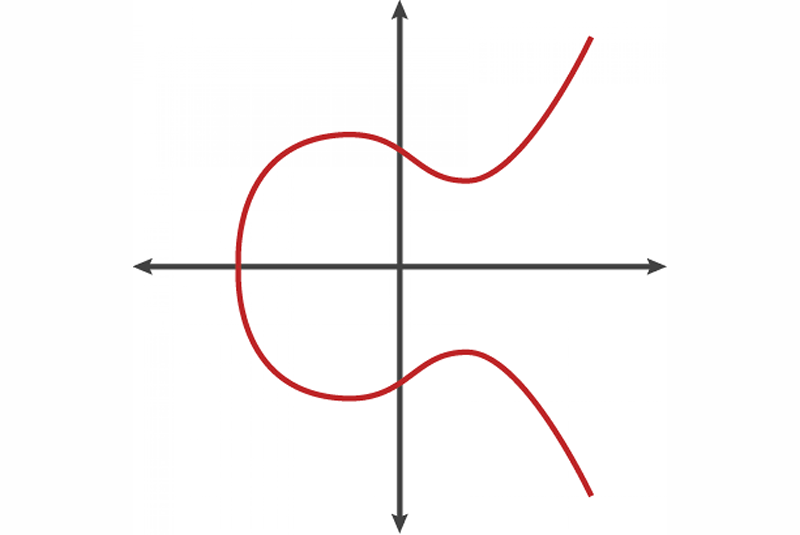
\includegraphics[width=\textwidth,height=0.5\textwidth]{fig01}
\caption{Elliptic Curve Cryptography representation}
\label{fig:01}
\end{figure}

It can create more minor, faster, and more efficient cryptographic keys. Instead of using a traditional method to generate products of huge prime numbers, it uses an elliptic curve equation to generate keys. ECC is used in all fundamental blockchain cryptocurrencies, and one of the well-known is Bitcoin. For hackers, it is hard to crack the ECC algorithm that works on the Elliptic Curve Discrete Logarithm Problem (ECDLP). Because of the mathematical specifics of ECC and the size of numbers needed to create an ECC key pair, the conclusion can be made that ECC is more compliant with the possibility of present RINGs.

Here is a quick comparison between RSA and ECC.

\begin{center}
\begin{tabular}{ | m{6cm} | m{6cm} | }
\hline
RSA & ECC \\
\hline
It has a slow algorithm, and it may make maximum use of computer resources such as batteries, etc. & The algorithm is fast as key sizes are smaller, less burden on system resources. \\
\hline
It is vulnerable to quantum computers and brute force attacks. & It uses the ECC algorithm that works on the Elliptic Curve Discrete Logarithm Problem (ECDLP). It is hard for hackers to crack it, making it much more secure. \\
\hline
In RSA, longer keys may be required for higher security. & Thanks to its shorter key lengths, ECDSA offers much better performance than RSA. \\
\hline
In RSA, scalability could be more optimal. & Scalability is improved as the server can handle higher traffic because of lower overhead. \\
\hline
RSA is more RNG limits dependent & Smaller keys, and mathematic specifics make ECC more secure in current RNG possibilities \\
\hline
\end{tabular}
\end{center}

\subsection{Through the time and Quantum computers}
\label{sub-sec:6-3}

Both algorithms (RSA, ECC) are relatively easy to hack, but all of them will change with the possible (and probable) introduction of quantum computers. The National Institute of Standards and Technology (NIST) predicts that modern public key cryptography will fail once quantum computing becomes mainstream. Quantum computers are mightily powerful — significantly more powerful than supercomputers nowadays — because they operate on qubits rather than bits. This means that they can try multiple combinations at any given time and, therefore, their computing time is significantly shorter. These quantum computers will likely make modern encryption systems, - including RSA and ECDSA.

\section{Conclusions}
\label{sec:7}

The study of the presented weaknesses in the asymmetric RSA algorithm is of high importance for a more secure and fast transition to the modern digital transformation. Hardware solutions that could significantly support the quality of RNG in computer systems have been listed, which would significantly affect the security of modular cryptography. The study also reveals RSA's cryptographic security problems when using it. This would lead to searching for a replacement of modular cryptography with other more secure solutions using the widespread computer systems RNG solutions.

\begin{thebibliography}{8}

\bibitem{01} Arjen K. Lenstra, James P. Hughes, Maxime Augier, Joppe W. Bos, Thorsten Kleinjung, Christophe Wachter: Ron was wrong, Whit is right, https://eprint.iacr.org/2012/064.pdf (2012)

\bibitem{02} Kerry Scharfglass, Darrin Weng, Joseph White, Christopher Lupo, Breaking weak 1024-bit RSA keys with CUDA, https://digitalcommons.calpoly.edu/cgi/viewcontent.cgi? referer=https://scholar.google.com/\&httpsredir=1\&article=1241\&context=csse\_fac

\bibitem{03} Cloostermans B., Quasi-linear GCD computation and factoring RSA moduli, Eindhoven University of Technology, Department of Mathematics and Computer Science, Bachelor Mathematics (2012)

\bibitem{04} Heninger N., Durumeric Z., Wustrow E., Halderman J. A., Mining Your Ps and Qs: Detection of Widespread Weak Keys in Network Devices, 21 st Security Symposium Security’12, ISBN 978-931971-95-9, Bellevue, WA, pp. 205—220 (2012)

\bibitem{18} M. Preetha, M. Nithya, A STUDY AND PERFORMANCE ANALYSIS OF RSA ALGORITHM, IJCSMC, Vol. 2, Issue. 6, June 2013, pg.126 – 139, ISSN 2320–088X

\bibitem{19} Kerry Scharfglass, Darrin Weng, Joseph White, Christopher Lupo, "Breaking weak 1024-bit RSA keys with CUDA", California Polytechnic State University, Dec 2012, Publisher: IEEE, DOI: 10.1109/PDCAT.2012.58 ISBN: 978-0-7695-4879-1

\bibitem{05} Li C., Zhang J., Sang L., Gong L., Wang L., Wang A., Wang Y., Deep Learning- Based Security Verification for a Random Number Generator Using White Chaos, Entropy, 22, 1134; doi:10.3390/e22101134 (2020)

\bibitem{06} Singh S., Maakar S. K. and Kumar S., A Performance Analysis of DES and RSA Cryptography, International Journal of Emerging Trends \& Technology in Computer Science (IJETTCS), Volume 2, Issue 3, ISSN 2278-6856 (2013)

\bibitem{07} Velizar Shalamanov, Vladimir Monov, Ivaylo Blagoev, Silvia Matern, Gergana Vassileva, Ivan Blagoev, A Model of ICT Competence Development for Digital Transformation. ISSN 0861-5160 (print), ISSN 1314-2119 (online) (2020)

\bibitem{20} Jang-Jaccard J., Nepal S., A survey of emerging threats in cybersecurity. Journal of Computer and System Sciences, 80(5), 973-993 (2014)

\bibitem{08} Xin Zhou and Xiaofei Tang, "Research and implementation of RSA algorithm for encryption and decryption," Proceedings of 2011 6th International Forum on Strategic Technology, Harbin, Heilongjiang, 2011, pp. 1118-1121, doi: 10.1109/IFOST.2011.6021216.

\bibitem{09} Kostadinov G., Atanasova T., Security Policies for Wireless and Network Infrastructure. Problems of Engineering Cybernetics and Robotics, vol. 71, 14-19, Bulgarian Academy of Sciences (2019)

\bibitem{10} Dineva, K., Atanasova, T.: Regression Analysis on Data Received from Modular IoT System. ESM’2019, EUROSIS-ETI, ISBN: 978-9492859-09-9, EAN: 9789492859099, pp.114-118, 2019

\bibitem{11} DiCarlo D., Random Number Generation: Types and Techniques, Liberty University, (2012)

\bibitem{12} Jin, A., Ling, D., Goh A., Biohashing: Two factor authentication featuring fingerprint data and tokenised random number. Pattern Recognition, 37, 2245- 2255. (2004)

\bibitem{13} Ergün S., Security analysis of a chaos-based random number generator for applications in cryptography, 15th International Symposium on Communications and Information Technologies (ISCIT), pp. 319-322, doi: 10.1109/ISCIT.2015.7458371 (2015)

\bibitem{14} Ryabko B., Astola J., Malyutov M., Compression-Based Methods of Statistical Analysis and Prediction of Time Series, Springer International Publishing Switzerland, eBook ISBN 978-3-319-32253-7 (2016)

\bibitem{15} Trappe, L., Washington, L. Introduction to cryptography with coding theory (2nd ed). Upper Saddle River, NJ: Pearson (2006)

\bibitem{16} Hart J. D., Roy R. and Murphy T. E., Optical random number generation - harvesting entropy from noise and chaos, 51st Annual Conference on Information Sciences and Systems (CISS), doi: 10.1109/CISS.2017.7926165 (2017)

\bibitem{17} Lavasani, A., Eghlidos, T. Practical next bit test for evaluating pseudo-random sequences. Scientia Iranica, 16(1), 19-33 (2009)

\bibitem{21} Dichtl, M. How to predict the output of a hardware random number generator. CHES 2003, 2779, 181-188. (2003) Dichtl, M. How to predict the output of a hardware random number generator. CHES 2003, 2779, 181-188. (2003).

\bibitem{22} Carr J., Simple random number generation, Computers \& Geosciences, 29(10):1269-1275 (2003).

\bibitem{23} L’Ecuyer P., Random Number Generation, In book: Handbook of Simulation: Principles, Methodology, Advances, Applications, and Practice (2007)

\bibitem{24} Camara C., Martín H., Peris-Lopez P., Aldalaien M., Design and Analysis of a True Random Number Generator Based on GSR Signals for Body Sensor Networks, Sensors 19, 2033; doi:10.3390/s19092033 (2019)

\end{thebibliography}
\end{document}
